\documentclass[11pt]{article}
\usepackage{graphics}
\usepackage{amsthm}
\usepackage{amsmath}
\usepackage{amssymb}
\usepackage{bm}
\usepackage{amsbsy}
\usepackage{mathtools}
\usepackage{algpseudocode, algorithm, algorithmicx}
\usepackage{soul}
\usepackage{graphicx}
\usepackage{color}
\usepackage{float}
\usepackage{gensymb}
\usepackage{tabularx}
\newcommand{\ord}[1]{\textsuperscript{#1}}
\usepackage{ragged2e}
\DeclareMathOperator{\DICT}{DICT}


\graphicspath{ {images/HW5/} }


\makeatletter
\newcommand\multiline[1]{\parbox[t]{\dimexpr\linewidth-\ALG@thistlm}{#1}}
\makeatother
\usepackage[margin=1in]{geometry}
%\renewcommand{\baselinestretch}{1.2}
\newcommand{\codepar}[2]{\begin{minipage}[t]{#1}#2\end{minipage}}
\newcommand{\codecomt}[1]{\color{blue}\textit{// #1}\color{black}}

% You can put more user-defined commands here

\makeatletter
\newlength{\continueindent}
\setlength{\continueindent}{6em}

\renewenvironment{algorithmic}[1][0]%
   {%
   \edef\ALG@numberfreq{#1}%
   \def\@currentlabel{\theALG@line}%
   %
   \setcounter{ALG@line}{0}%
   \setcounter{ALG@rem}{0}%
   %
   \let\\\algbreak%
   %
   \expandafter\edef\csname ALG@currentblock@\theALG@nested\endcsname{0}%
   \expandafter\let\csname ALG@currentlifetime@\theALG@nested\endcsname\relax%
   %
   \begin{list}%
      {\ALG@step}%
      {%
      \rightmargin\z@%
      \itemsep\z@ \itemindent\z@ \listparindent2em%
      \partopsep\z@ \parskip\z@ \parsep\z@%
      \labelsep 0.5em \topsep 0.2em%\skip 1.2em 
      \ifthenelse{\equal{#1}{0}}%
         {\labelwidth 0.5em}%
         {\labelwidth 1.2em}%
       \leftmargin\labelwidth \addtolength{\leftmargin}{\labelsep}
      \ALG@tlm\z@%
      }%
      \parshape 2 \leftmargin \linewidth \continueindent \dimexpr\linewidth-\continueindent\relax
   \setcounter{ALG@nested}{0}%
   \ALG@beginalgorithmic%
   }%
   {% end{algorithmic}
   % check if all blocks are closed
   \ALG@closeloops%
   \expandafter\ifnum\csname ALG@currentblock@\theALG@nested\endcsname=0\relax%
   \else%
      \PackageError{algorithmicx}{Some blocks are not closed!!!}{}%
   \fi%
   \ALG@endalgorithmic%
   \end{list}%
   }%
\makeatother

\newcommand{\CH}{\mathrm{CH}}
\renewcommand{\thealgorithm}{}

\newenvironment{solution}
  {\renewcommand\qedsymbol{$\blacksquare$}\begin{proof}[Solution]}
  {\end{proof}}
  
\begin{document}

\hrule
\begin{center}
    \textbf{CS91T: Computational Geometry}\hfill \textbf{Fall 2023}\newline

    {\Large Homework 5}

    David Yang and Nick Fettig
\end{center}

\hrule

\vspace{1em}


\begin{enumerate}
\item\textbf{Let’s (temporarily) define the quality of a polygon triangulation to be the minimum interior angle of any triangle used. A high-quality triangulation must avoid sliver triangles, so maximizing quality seems related to the goal of minimizing cost (in the sense of total length of diagonals). Using an explicit example, prove that these two goal are not equivalent.}

\begin{center}
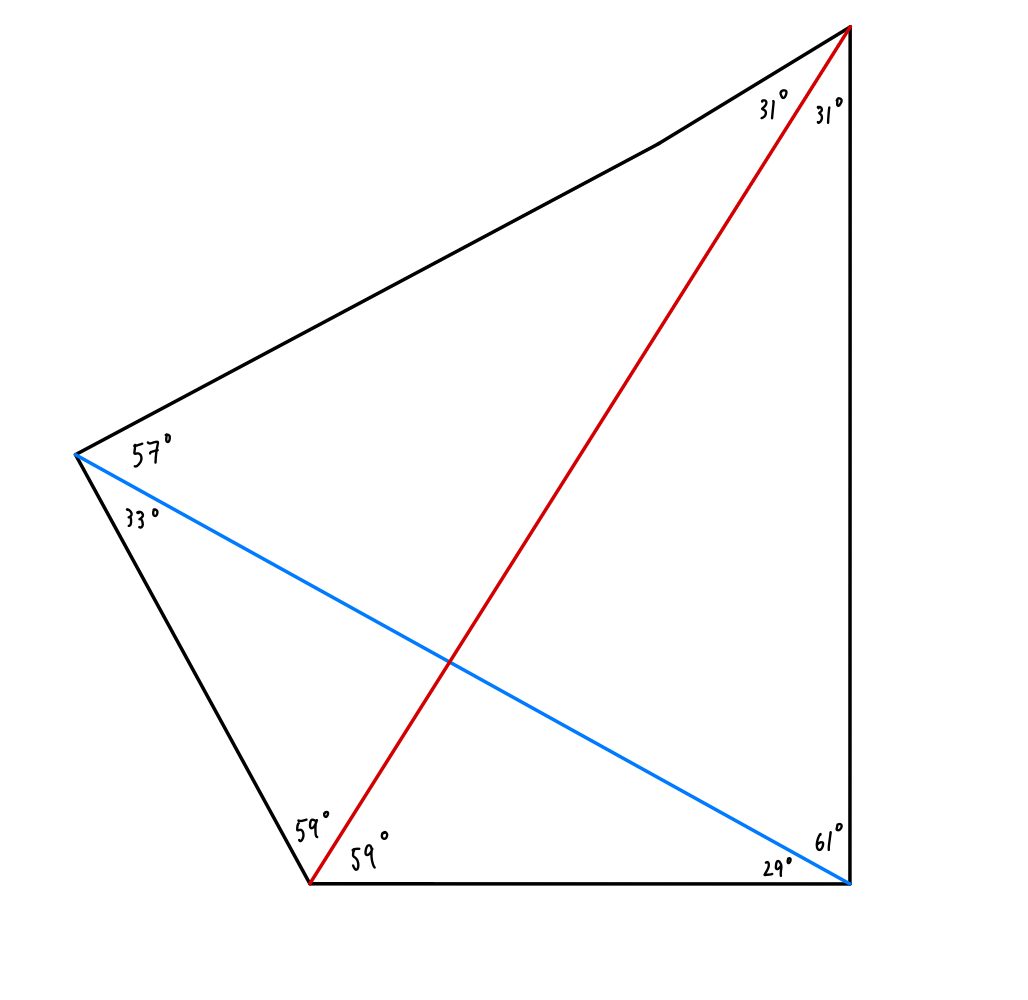
\includegraphics[scale=0.25]{images/HW5/CS91.HW5.1.jpeg}
\end{center}

\begin{solution}
The above construction is a counterexample to the statement that minimizing cost (in the sense of total length of diagonals) is equivalent to maximizing quality (in the sense of the minimum interior angle of any triangle used). \\

The blue diagonal is the minimum length triangulation, and thus, it is the triangulation that minimizes the cost. However, the red diagonal is the maximum quality triangulation since the minimum interior angle in the red triangulation is $31^{\circ}$ compared to $29^{\circ}$ in the case of the blue triangulation. \\

Since these two goals yield different triangulations in the above example, they are not equivalent.
\end{solution}
\newpage
\item\textbf{On $n$ parallel railway tracks there are $n$ trains going at constant speeds $v_1,\dots,v_n$. At time
$t = 0$, the trains are at positions $k_1,\dots, k_n$. Using the algorithm for computing intersections of half-planes, design an $O(n \log n)$-time algorithm that lists all trains that are ever in the lead.} \\


Assume we are given the initial train speeds and positions in the form of $n$-length arrays (indexed from $1$), $V$ and $K$, respectively. Assume we are also provided a bounding box of (a very large) size $M$.

\begin{minipage}[t]{0.9\textwidth}
    \begin{algorithm}[H]
    \caption{\textsc{GetTrainsInLead}($V, K, M, n$)}
    \begin{algorithmic}[1]
        \State{Set $ret$ to an empty set}
        \State{Set $\ell$ to an empty array of size $n$ to hold lines}
        \For{\textbf{each} $i \in \{1, \dots, n\}$}
            \State{Set $\ell[i]\coloneqq$ a line of slope $V[i]$ through $(0, K[i])$ and bounded between $[0, M]^2$ }
        \EndFor
        \State{Set $intersection\coloneqq$ \textsc{IntersectionOfHalfPlanes($\ell$)}\footnotemark}
        \For{\textbf{each} $vertex$ in $intersection$}
            \State{Add the line indices of $vertex$ to $ret$}
        \EndFor
        \State{\textbf{return} $ret$}
    \end{algorithmic}
    \end{algorithm}
\end{minipage}

\vspace{1cm}

\footnotetext{\textsc{IntersectionOfHalfPlanes} finds the intersection of all upper half planes of a provided list of lines ($\ell$). The function will return a list of the vertices that form the convex polygon created by the intersection of half-planes. Assume that each vertex holds the indices of the lines in $\ell$ that form it.}

\textbf{Algorithm Explanation}: Our algorithm creates a set of lines that give context to their position over time. These lines are bounded by a large box $[0, M]^2$ to make computation easier. The algorithm then calls \textsc{IntersectionOfHalfPlanes}, a helper function to find the intersection of the upper half-planes of a list of lines. The return value is a list of the vertices that form the convex polygon of the intersection. These vertices have the extra condition that they hold information on the two lines (train indices) that form them. We add both of the line indices associated with each vertex to a set as those trains are at some point in the lead, and return this set. \\

\textbf{Runtime Analysis}: Lines 1-2 initialize two variables used in our algorithm, in $O(1)$ time. The first for loop on lines $3-5$ runs $n$ times to create a line corresponding to each train. Creating a line and adding it to our list, $\ell$, both take $O(1)$ time. On line 6, we call \textsc{IntersectionOfHalfPlanes}, a helper function that uses the divide-and-conquer algorithm discussed in class to find the intersection of the upper half planes of each line in $\ell$. This algorithm takes $O(n\log n)$ time to run. The second loop in lines 7 to 9 runs for each vertex in the convex polygon formed by the intersection of the half-planes. There are at most $n+2$ vertices in $intersection$: one for each of the $n$ trains and two more due to the large bounding box of size $M$. Adding the line indices of each vertex to $ret$ takes $O(1)$ time. Therefore, the total running time is

\[O(1) + O(n) \cdot O(1) + O(n\log n) + O(n+2) \cdot O(1) = O(n\log n)\]

as desired. \\

\textbf{Proof of Correctness}: Our algorithm works given the context in which the lines are created and evaluated. We are essentially constructing a position vs. time graph, where the lines represent the position of each train over time: their $y$-intercept represents their initial position and their slope represents their speed. \\

For a train to be in the lead at a given time, every other train must have a smaller position at that time. Equivalently, the half-plane of every other train (represented by a line) will encompass a part of the line of the train in the lead. Therefore, the boundary of the intersection of all upper half-planes of the lines represents the trains that were at some point in the lead. \\

Our algorithm creates this ``graph" by plotting each train as a line with the correct initial position and slope. To find the intersection of half-planes of the train lines, we can assume \textsc{IntersectionOfHalfPlanes} works. Because each vertex holds information on the lines (trains) that form it, we will correctly determine all trains that were in the lead at some point in time, as desired.

\newpage
\item\textbf{(From Dasgupta, Papadimitriou, and Vazirani) A certain string-processing language offers a primitive operation which splits a string into two pieces. Since this operation involves copying the original string, it takes $n$ units of time for a string of length $n$, regardless of the location of the cut. Suppose, now, that you want to break a string into many pieces. The order in which the breaks are made can affect the total running time. For example, if you want to cut a $20$-character string at positions $3$ and $10$, then making the first cut at position $3$ incurs a total cost of $20 + 17 = 37$, while doing position $10$ first has a better cost of $20 + 10 = 30$. Give an $O(m^3)$-time dynamic programming algorithm that, given the locations of $m$ cuts in a string of length $n$, finds the minimum cost of making those $m$ cuts.} \\

For preprocessing, let us create a length $m+2$ array, $cuts$, which stores the location of the $m$ cuts in order of their location from left to right, in indices $1$ to $m$, and set $cuts[0] = 0$ and $cuts[m+1] = n$. We will pass the array $cuts$, and the length of the string, $n$, into the following algorithm.

\begin{minipage}[t]{0.9\textwidth}
    \begin{algorithm}[H]
    \caption{\textsc{MinimumCutCost}($cuts, n$)}
    \begin{algorithmic}[1]
        \State{Set $m = cuts.length() - 2$}
        \State{Initialize $string$ to be an empty $(m + 2) \times (m+2)$ length array.}
        \For{$i \in \{0, \dots, m+1\}$}
        \For{$j \in \{0, \dots, m+1\}$}
            \If{$j = i$ or $j = i + 1$}
                \State{Set $string[i][j] = 0$.}
            \Else
                \State{Set $string[i][j] = \infty$.}
            \EndIf
        \EndFor
        \EndFor
        \For{$idx \in \{ m + 1, \dots, 0\}$}
        \For{$sep \in \{0, \dots, m + 1\}$}
            \If{$idx + sep < m + 2$}
               \State{Set $string[idx][idx + sep] = \min \limits_{idx < j < idx + sep} \{ string[idx][j] + string[j][idx + sep] + cuts[idx + sep] - cuts[idx]\}.$}      
            \EndIf

        \EndFor
        \EndFor
        \State{\textbf{return} $string[0][m+1]$}
    \end{algorithmic}
    \end{algorithm}
\end{minipage}

    \vspace{1cm}

    \textbf{Algorithm Explanation}: The entry $string[idx1][idx2]$, where $0 \leq idx1, \, idx2 \leq m+1$ stores the minimum cost required to handle all cuts between $idx1$ and $idx2$, exclusive, where $idx1$ and $idx2$ refer to the indices of the respective cuts in the $cuts$ array (in this problem, we only care about entries where $idx1 \leq idx2$, and other entries remain set at $\infty$). We return $string[0][m+1]$ since we want the minimum cost of making all $m$ cuts (corresponding to indices $1$ to $m$) on the given string of length $n$. \\

    The $sep$ variable stores the separation between the pairs of cut indices we consider, whereas $idx$ stores the index of the current cut we are considering. \\
    
    To explain the iteration order, note that in line $12$, $idx$ starts at $m+1$ and decrements until $0$ to ensure that we calculate the minimum costs in the correct order (the minimum cost for a sequence of cuts starting at a lower index requires the correct minimum cost for a sequence of cuts starting at the larger indices). The remainder of the algorithm and its correctness are discussed in the proof of correctness section.\\

    
    \textbf{Runtime Analysis}: Lines $1$ to $11$ consist of basic initialization. The initialization of the $string$ array in line $2$ requires $O(m^2)$ time. Then, in lines $3$ to $11$, we iterate over every element to set them to $0$ or $\infty$, depending on a condition that can be checked in $O(1)$ time. These steps, in total, take $O(n^2)$ time. Lines $12$ to $18$ consist of the bulk of the algorithm; our two outer for loops in lines $12$ and $13$ require $O(m)$ time each, and our update condition in line $15$ requires iterating through all possible indices $j$ between $idx$ and $idx+sep$, for an additional factor of $O(m)$ iterations. Consequently, entire loop runs in $O(m)^3 = O(m^3)$ time. The final return statement in line $19$ takes $O(1)$ time, and thus, our dynamic programming algorithm runs in $O(m^3)$ time, as desired. \\

    \textbf{Proof of Correctness}: We will prove the correctness of our algorithm using strong induction on the value of the $sep$ variable; namely, our algorithm properly calculates the minimum cost of making cuts separated by $sep$ positions when sorted from left to right. Note that by construction, our algorithm properly handles the minimum cost when $sep = 0$ or $1$; since there are no cuts between two of the same cuts, or consecutive cuts, the minimum cost to handle the cuts between two cuts separated by $sep = 0 \text{ or } 1$ is simply $0$. \\

    For our inductive hypothesis, assume that our algorithm correctly calculates the minimum cost for any two cuts separated by $\leq k$ positions. We will show that the algorithm also correctly calculates the minimum cost for any two cuts separated by $sep = k+1$ positions. Consider any sequence of cuts that handles all cuts between two indices $i_1, i_2$ separated by $k+1$ cuts. In this sequence of cuts, there is a first cut between these two indices, at some position $p$ between $i_1$ and $i_2$, satisfying $i_1 < p < i_2$. By definition, the cost of the entire sequence of cuts between the two initial indices, then, is the cost of the first cut at index $p$, which is the distance between the initial two indices, plus the minimum cost to cut everything from indices $i_1$ to $p$ and $p$ to $i_2$. The process of going through each potential index $p$ is precisely the update step in line $15$. \\
    
    Since the separation between $i_1$ and $p$ and $p$ to $i_2$ are each less than or equal to $k$, they are already properly handled by the inductive hypothesis, and thus, by iterating through all possible positions $p$, we will find the minimum cost for any two cuts separated by $sep = k+1$ positions. \\
    
    Thus, by induction, our dynamic programming algorithm will find the minimum cost of making the given $m$ cuts on a string of length $n$, as desired.

    \newpage

    \item \textbf{Prove that $\Omega(n \log n)$  is a lower bound on the worst-case time complexity of finding all optimal solutions to a three-dimensional linear program with n constraints. Your proof should use the technique of reduction from sorting, just like our $\Omega(n \log n)$ lower bound on finding the convex hull of $n$ points in the plane. That is, you should explain how, given an unsorted array $A$ of length $n$, you could sort $A$ by constructing a three-dimensional linear program with $O(n)$ constraints (in $O(n)$ time), finding all solutions to that LP, and then post-processing the solutions (in $O(n)$ time) to get a sorted version of $A$.} 

    \begin{solution}
    In the following procedure, we will use a reduction from sorting. Begin with an unsorted array $A$ of length $n$. Take the $\arctan$ of each entry of $A$. Now, the $i^{\text{th}}$ entry (where $i \in \{1, 2, \dots, n\})$ in this array is simply an angle $\theta_i \in (-\frac{\pi}{2}, \frac{\pi}{2})$, as this is the range of the $\arctan$ function. \\

    For each entry, define the line \[\ell_i = -\cot \theta_i (x - \cos \theta_i) + \sin \theta_i,\] where $\ell_i$ is the tangent line to the point $p_i = (\cos \theta_i, \sin \theta_i)$ on the unit circle, which has angle $\theta_i$ relative to the positive $x$-axis. \\

    We construct a three-dimensional\footnote{we are really constructing a two-dimensional linear program, but we can trivially add constraints to set our third variable to $0$} linear program with:
    \begin{itemize}
        \item trivial optimization function (constant).
        \item linear constraints $c_i$, for each $i \in \{1, \dots, n\}$, representing the half-plane of $\ell_i$ containing the origin
        \item the additional linear constraint $x \geq 0$, to bound the resulting feasible region in the positive $x$-axis
    \end{itemize}

    Clearly, this is a three-dimensional linear program with $n + 1 = O(n)$ constraints (one for each entry in $A$). Furthermore, the solution to the linear program will be the vertices of the polygon enclosed by the tangent lines $\ell_i$, in clockwise order. \\

    We now must recover the sorted order of the original elements of $A$ using the solution to the linear program. To do this, iterate through the solution of the LP (corresponding to vertices of the polygon). Take consecutive vertices (in clockwise order), and compute the slope between them. Since the slope between these vertices is simply the slope $\cot \theta_i$ of some line $\ell_i$, we can recover $\theta_i$ by calculating the inverse cotangent of this slope. Finally, we apply $\tan \theta_i$ to recover the initial element of $A$. Iterating through the vertices in clockwise order and applying these inverse functions will allow us to recover the initial elements of $A$, in sorted order, as desired. \\

    Thus, by a reduction from sorting, which runs in $\Omega(n \log n)$, we know that $\Omega(n \log n)$  is a lower bound on the worst-case time complexity of finding all optimal solutions to a three-dimensional linear program with n constraints, as desired.
    \end{solution}

\end{enumerate}
\end{document}